\documentclass[12pt,a4paper]{article}
\usepackage{geometry}
\usepackage[numbers]{natbib}
\usepackage{amssymb, amsmath}
\usepackage{graphicx}
\usepackage{grffile}
\graphicspath{{../Figures/}}
\usepackage{gensymb}
\usepackage[font=small]{caption}
\usepackage[utf8]{inputenc}
\usepackage[english]{babel}
\usepackage{fancyhdr}
\usepackage[raggedright]{titlesec}
\usepackage{subcaption}
\usepackage{multirow}
\usepackage{dirtytalk}
\usepackage{framed}
\usepackage[pdftex,breaklinks]{hyperref}
\hypersetup{
  colorlinks   = true, %Colours links instead of ugly boxes
  urlcolor     = green, %Colour for external hyperlinks
  linkcolor    = blue, %Colour of internal links
  citecolor   = red %Colour of citations
}


\begin{document}
\author{Katrina Ashton}


\pagestyle{fancy}
\fancyhf{}
\rhead{\thepage}
\lhead{u5586882}

\section{What I've done}
\begin{itemize}
\item{Modified code to capture the RGB image associated with each point cloud}
\item{Investigated boxes (except for the checkered one) to see if they were getting picked up by the RealSense}
%\item{Added more to the appendices for the final report draft}
\end{itemize}

\section{Parts of report to look at}
\begin{itemize}
\item{Nothing new.}
\end{itemize}

\section{Questions}
\begin{itemize}
\item
\end{itemize}

\section{Comments}
\begin{itemize}
\item I need to fix up the file naming system before collecting more data as MATLAB gets them in the wrong order.
\end{itemize}

\section{Box Visibility Investigation}
\textbf{Purpose} \\
To investigate which boxes should be used to construct the scene and see if any other possible problems with data collection can be identified.
\\\\
\textbf{Set-up} \\
Place the first box to be investigated in the center of the flying space, with the Vicon off. Connect up the battery for the quadcopter and ssh into the TX2. 
\\\\
\textbf{Method} \\
Place the quadcopter at approximately 1.5m away from the box (facing towards it) and start the data capture program via ssh. Lift the quadcopter up to 1.5m, and ensure that the camera is pointing at the box. Pause for a few seconds, then slowly start moving the quadcopter towards the box, decreasing height as you move forwards so that the camera remains pointing at the box. Once you reach approximately 0.65m away from the box, slowly move the quadcopter back along the same trajectory until it reaches the starting position.
\\\\
Switch angle of quadcopter so that the RealSense is at an angle of 90 degrees with the box and bring the quadcopter close to the ground so that the RealSense is pointing at the box. Repeat the previous step, but keep the quadcopter at the same height.
\\\\
Repeat for the other two boxes, stopping the data capture between switches (unplug and re-plug the RealSense if necessary to get the data capture program to work). Then repeat the previous steps with the Vicon turned on.
\\\\
\textbf{Results} \\
Box 1: Square, black with small white label, not shiny. \\
\begin{figure}[h]
  \begin{subfigure}[t]{0.5\textwidth}
  \centering
    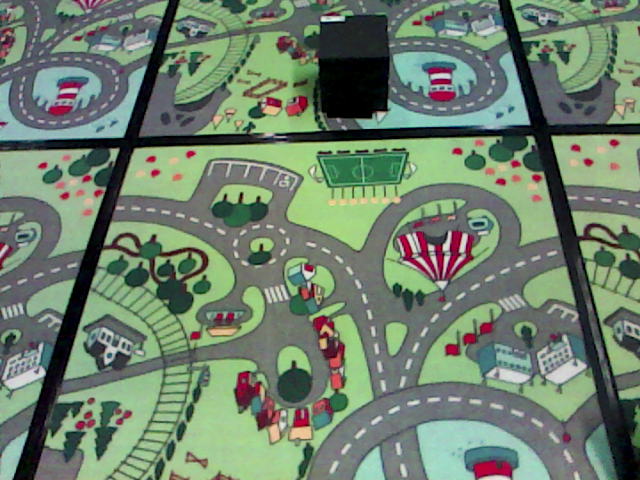
\includegraphics[width=60mm]{box_test/cpp-headless-output-118_4_16_1_57_40_1526435860119.png}
  \caption{RGB-D image}
  \end{subfigure}%
  ~
  \begin{subfigure}[t]{0.5\textwidth}
  \centering
    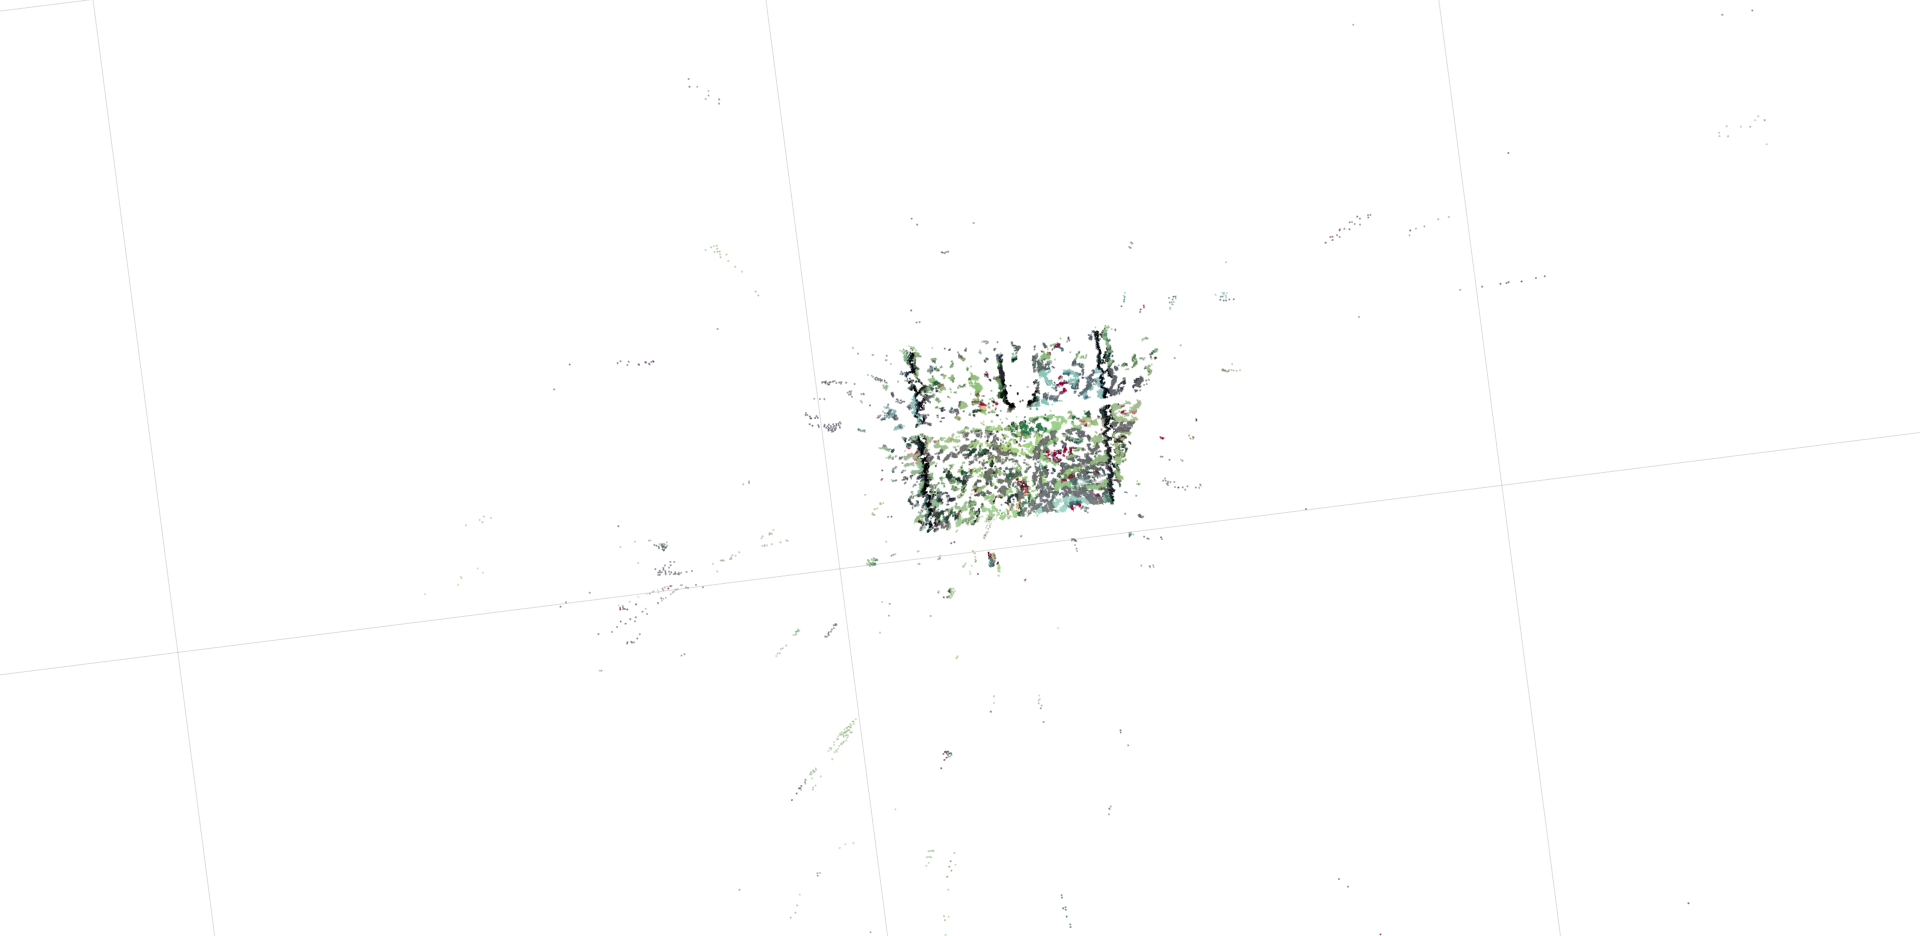
\includegraphics[width=60mm, trim =230mm 100mm 200mm 70mm, clip]{box_test/no_vicon1_36.png}
  \caption{Point cloud}
  \end{subfigure}
  \caption{RGB Image and Point cloud for box 1, 45 degree angle.}
\end{figure}

\noindent
The vertical edges of the box are visible, but the rest is not. \\
Also note that some of the tape can be seen (at the sides) but the horizontal strip is not visible.
\\\\
\newpage
\noindent
Box 2: Rectangular placed lengthwise, brown with black Dell logo in the middle, not shiny. \\
\begin{figure}[h]
  \centering
  \begin{subfigure}[t]{0.5\textwidth}
  \centering
    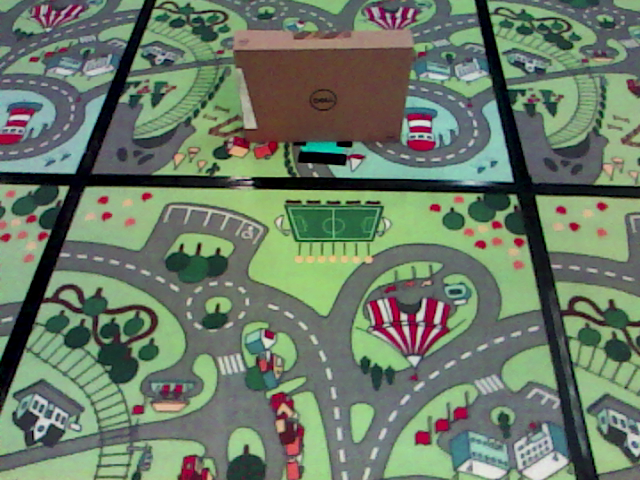
\includegraphics[width=60mm]{box_test/cpp-headless-output-118_4_16_1_59_18_1526435958825.png}
  \caption{RGB-D image}
  \end{subfigure}
  \\
  \begin{subfigure}[t]{0.4\textwidth}
  \centering
    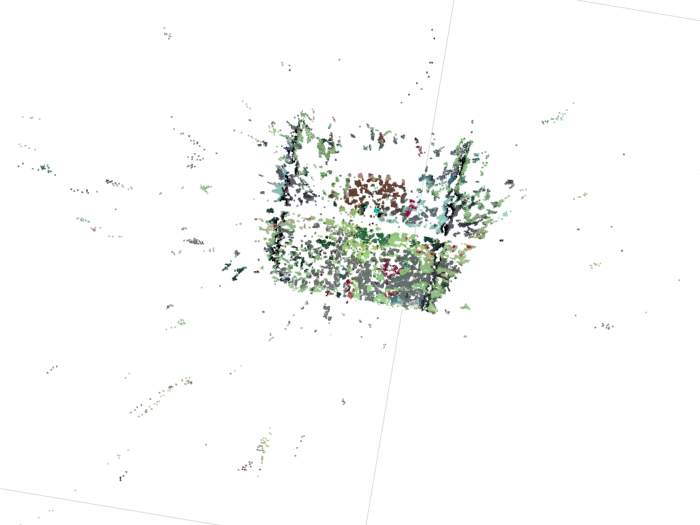
\includegraphics[width=60mm, trim =70mm 50mm 50mm 10mm, clip]{box_test/no_vicon1_161_flat.png}
   \caption{Point cloud, top view}
   \end{subfigure} % 
   ~
  \begin{subfigure}[t]{0.4\textwidth}
  \centering
    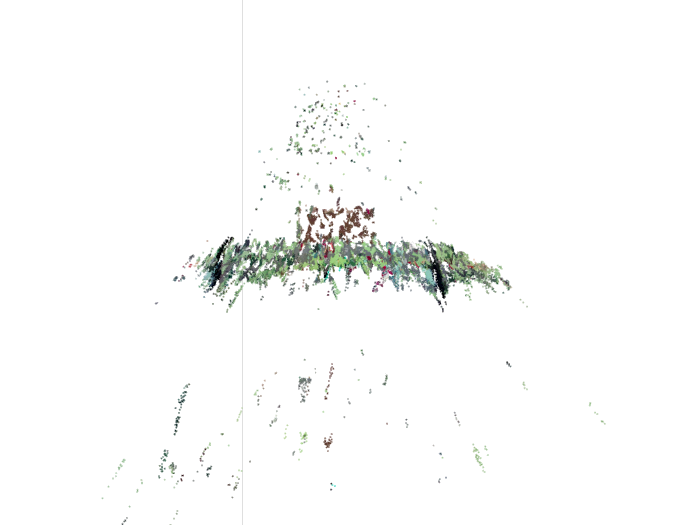
\includegraphics[width=60mm, trim =50mm 50mm 50mm 0mm, clip]{box_test/no_vicon1_161.png}
  \caption{Point cloud, side view}
  \end{subfigure}
  \caption{RGB Image and Point cloud for box 2, 45 degree angle.}
\end{figure}

\noindent
The brown box is clearly visible, with points over the whole object, however it is very patchy.
\\\\
\newpage
\noindent
Box 3: Rectangular placed on short edge, black with yellow stripe, shiny. \\
\begin{figure}[h]
  \begin{subfigure}[t]{0.5\textwidth}
  \centering
    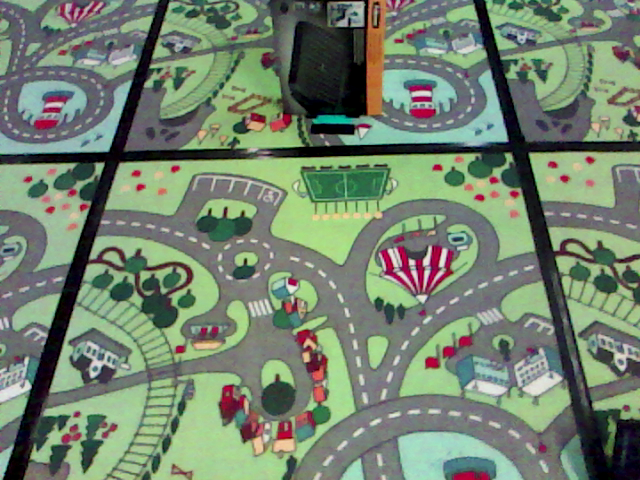
\includegraphics[width=60mm]{box_test/cpp-headless-output-118_4_16_2_0_59_1526436059005.png}
  \caption{RGB-D image}
  \end{subfigure}%
  ~
  \begin{subfigure}[t]{0.5\textwidth}
  \centering
    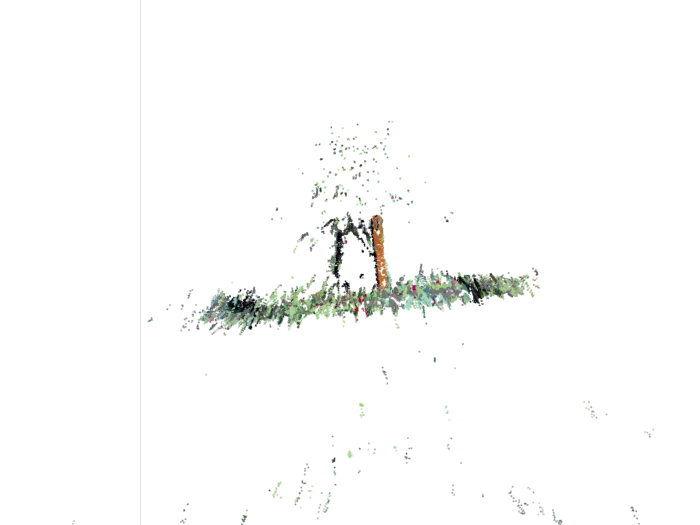
\includegraphics[width=60mm, trim =50mm 50mm 50mm 50mm, clip]{box_test/no_vicon1_281.png}
  \caption{Point cloud}
  \end{subfigure}
  \caption{RGB Image and Point cloud for box 1, 45 degree angle.}
\end{figure}

\noindent
The yellow part of the box is fairly visible, as is the other vertical edge. However the center part is completely missing.
\\\\
Impact of Vicon \\
\begin{figure}[h]
  \centering
    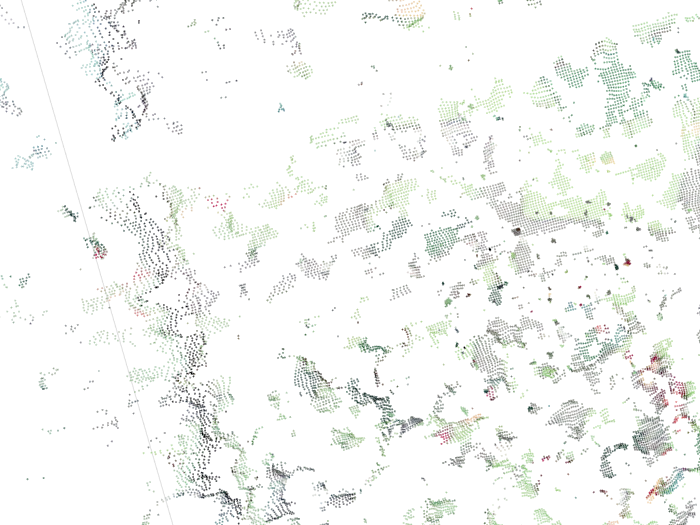
\includegraphics[width=60mm]{box_test/no_vicon1_36_wave.png}
  \caption{Point cloud with waves, obtained with no Vicon}
  \label{f: no vicon waves}
\end{figure}

\noindent
The wave pattern that can be seen by zooming in on a point cloud is present even without the Vicon on.
\\\\
\textbf{Conclusion} \\
Part of the issue may be the field of view, as currently the middle of the frame should be at the origin on the ground, so the tops of the boxes may get cut-off. (The RGB images should be used to confirm if this is happening during the flight when the quadcopter is controlled by the Vicon, as this experiment only used approximate distances).
\\\\
More texture should be added to the black and brown box to allow them to be picked up better by the RealSense or they should be replaced with more textured boxes, boxes with large stretches of black should not be used.
\\\\
The Vicon does not seem to be negatively impacting the boxes being picked up as most of them do not show up well even when it is off. The wave pattern occurs even with the Vicon off.

\end{document}